\documentclass{beamer}

\usepackage[frenchb]{babel}
\usepackage[utf8]{inputenc}  
\usepackage[T1]{fontenc}
\usepackage[lined,ruled,boxed,linesnumbered]{algorithm2e}
\usepackage{amsmath,amsfonts,amsbsy,amssymb,mathabx,amsthm,bbm,bm} 
\usepackage{graphicx}
\usepackage{arydshln}
\usepackage{stmaryrd}

\usetheme{Warsaw}

\title{Les Codes LDPC}
\author{Banier Corentin et Karboul Maher}
\institute{Université de Bordeaux}
\date{18 Mai 2021}

\begin{document}
	\begin{frame}
    \titlepage
	\end{frame}

    \begin{frame}
        \frametitle{Introduction}
    \end{frame}

    \begin{frame}
        \frametitle{Définition d'un code LDPC}
    \end{frame}

    \begin{frame}
        \frametitle{Construction des codes LDPC}
        \framesubtitle{La construction de Gallager}
    \end{frame}
    
    \begin{frame}
        \frametitle{Construction des codes LDPC}
        \framesubtitle{Construction utilisée pour nos tests}
    \end{frame}

    \begin{frame}
        \frametitle{Algorithme de décodage}
        \begin{figure}[!h]
            \centering
            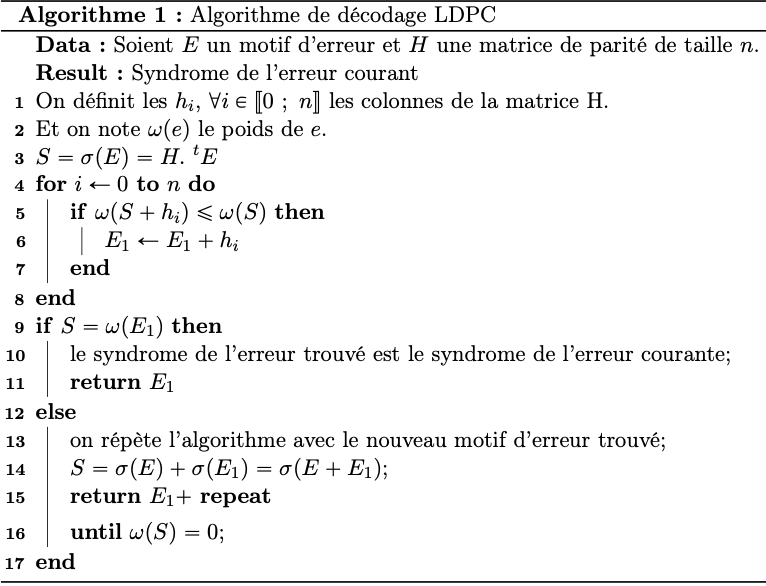
\includegraphics[scale=0.65]{algo.png}  
            \label{fig:algo}
        \end{figure}
    \end{frame}

    \begin{frame}
        \frametitle{Expérimentations}
    \end{frame}

    \begin{frame}
        \frametitle{Conclusion}
    \end{frame}

\end{document}